%%%%%%%%%%%%%%%%%%%%%%%%%%%%%%%%%%%%%%%%%
% Make sure to set your name, legi number and url to the right git branch.
\newcommand{\hmwkAuthorName}{Lin Zhang} % Your name
\newcommand{\hmwkAuthorLegi}{16-930-687} % Your name
\newcommand{\hmwkGitBranch}{https://gitlab.vis.ethz.ch/vwegmayr/slt-coding-exercises/tree/16-930-687/1\_locally\_linear\_embedding} % Your name
%
%%%%%%%%%%%%%%%%%%%%%%%%%%%%%%%%%%%%%%%%%

%----------------------------------------------------------------------------------------
%	PACKAGES AND OTHER DOCUMENT CONFIGURATIONS
%	Skip this
%----------------------------------------------------------------------------------------

\documentclass{article}

\usepackage{fancyhdr} % Required for custom headers
\usepackage{lastpage} % Required to determine the last page for the footer
\usepackage{extramarks} % Required for headers and footers
\usepackage{graphicx} % Required to insert images
\usepackage{lipsum} % Used for inserting dummy 'Lorem ipsum' text into the template

% Margins
\topmargin=-0.45in
\evensidemargin=0in
\oddsidemargin=0in
\textwidth=6.5in
\textheight=9.0in
\headsep=0.25in 

\linespread{1.1} % Line spacing

% Set up the header and footer
\pagestyle{fancy}
\lhead{\hmwkAuthorName} % Top left header
\chead{\hmwkClass\ \hmwkTitle} % Top center header
\rhead{\firstxmark} % Top right header
\lfoot{\lastxmark} % Bottom left footer
\cfoot{} % Bottom center footer
\rfoot{Page\ \thepage\ of\ \pageref{LastPage}} % Bottom right footer
\renewcommand\headrulewidth{0.4pt} % Size of the header rule
\renewcommand\footrulewidth{0.4pt} % Size of the footer rule

\setlength\parindent{0pt} % Removes all indentation from paragraphs

%----------------------------------------------------------------------------------------
%	DOCUMENT STRUCTURE COMMANDS
%	Skip this
%----------------------------------------------------------------------------------------

% Header and footer for when a page split occurs within a problem environment
\newcommand{\enterProblemHeader}[1]{
\nobreak\extramarks{#1}{#1 continued on next page\ldots}\nobreak
\nobreak\extramarks{#1 (continued)}{#1 continued on next page\ldots}\nobreak
}

% Header and footer for when a page split occurs between problem environments
\newcommand{\exitProblemHeader}[1]{
\nobreak\extramarks{#1 (continued)}{#1 continued on next page\ldots}\nobreak
\nobreak\extramarks{#1}{}\nobreak
}

\setcounter{secnumdepth}{0} % Removes default section numbers
\newcounter{homeworkProblemCounter} % Creates a counter to keep track of the number of problems

\newcommand{\homeworkProblemName}{}
\newenvironment{homeworkProblem}[1][Problem \arabic{homeworkProblemCounter}]{ % Makes a new environment called homeworkProblem which takes 1 argument (custom name) but the default is "Problem #"
\stepcounter{homeworkProblemCounter} % Increase counter for number of problems
\renewcommand{\homeworkProblemName}{#1} % Assign \homeworkProblemName the name of the problem
\section{\homeworkProblemName} % Make a section in the document with the custom problem count
\enterProblemHeader{\homeworkProblemName} % Header and footer within the environment
}{
\exitProblemHeader{\homeworkProblemName} % Header and footer after the environment
}

\newcommand{\problemAnswer}[1]{ % Defines the problem answer command with the content as the only argument
\noindent\framebox[\columnwidth][c]{\begin{minipage}{0.98\columnwidth}#1\end{minipage}} % Makes the box around the problem answer and puts the content inside
}

\newcommand{\homeworkSectionName}{}
\newenvironment{homeworkSection}[1]{ % New environment for sections within homework problems, takes 1 argument - the name of the section
\renewcommand{\homeworkSectionName}{#1} % Assign \homeworkSectionName to the name of the section from the environment argument
\subsection{\homeworkSectionName} % Make a subsection with the custom name of the subsection
\enterProblemHeader{\homeworkProblemName\ [\homeworkSectionName]} % Header and footer within the environment
}{
\enterProblemHeader{\homeworkProblemName} % Header and footer after the environment
}
   
%----------------------------------------------------------------------------------------
%	NAME AND CLASS SECTION
%	Skip this
%----------------------------------------------------------------------------------------

\newcommand{\hmwkTitle}{Locally Linear Embedding} % Assignment title
\newcommand{\hmwkDueDate}{Monday,\ March\ 6th,\ 2017} % Due date
\newcommand{\hmwkClass}{SLT coding exercise\ \#1} % Course/class
\newcommand{\hmwkClassTime}{Mo 16:15} % Class/lecture time
\newcommand{\hmwkClassInstructor}{} % Teacher/lecturer

%----------------------------------------------------------------------------------------
%	TITLE PAGE
%	Skip this
%----------------------------------------------------------------------------------------

\title{
\vspace{2in}
\textmd{\small{\hmwkClass}}\\
\textmd{\textbf{\hmwkTitle}}\\
\small{https://gitlab.vis.ethz.ch/vwegmayr/slt-coding-exercises}\\
\normalsize\vspace{0.1in}\small{Due\ on\ \hmwkDueDate}
%\vspace{0.1in}\large{\textit{\hmwkClassInstructor\ \hmwkClassTime}}
\vspace{3in}
}

\author{
\hmwkAuthorName\\
\hmwkAuthorLegi
}

\date{ } % Insert date here if you want it to appear below your name

\begin{document}

\maketitle

%----------------------------------------------------------------------------------------
%	TABLE OF CONTENTS
%	Skip this
%----------------------------------------------------------------------------------------

%\setcounter{tocdepth}{1} % Uncomment this line if you don't want subsections listed in the ToC

\newpage
\tableofcontents
\newpage

%----------------------------------------------------------------------------------------
%	SECTIONS
%	Now you are in the right hood
%----------------------------------------------------------------------------------------

\begin{homeworkProblem}[The Model]
The model section is intended to allow you to recapitulate the essential ingredients used in \hmwkTitle. Write down the \textit{necessary} equations to specify \hmwkTitle\ and and shortly explain the variables that are involved. This section should only introduce the equations, their solution should be outlined in the implementation section.\newline
Hard limit: One page
\vspace{10pt}

\problemAnswer{ % Answer
Locally linear embedding (LLM) is an unsupervised learning algorithm that computes low-dimensional neighbourhood preserving embeddings. Given $N$ real-valued vectors $x_i$ with the dimensionaly $D$. It is supposed that data point with its neighbourhoods lie on or close to a locally linear patch. We characterize the local goemetry of these patches by linear coefficients that reconstruct each data point from its neighbours. The reconstruction error is the sum of the squared distance between all the data points and their reconstructions: 
\begin{equation}
E(W)=\sum\limits_{i} (x_i-\sum\limits_{j}w_{ij} x_j)^2,
\end{equation}
whereas the weights $w_{ij}$ is the contribution of the j-th data point to the i-th reconstruction with the constraint $\sum\limits_{j}w_{ij}=1$.\\
With the fixed weights each high dimensional observation vector $x_i$ is mapped to a low dimensional vector $y_i$ with the dimensionality $d<<D$. We choose the coordinates $y_i$ to minimize the embedding cost function:
\begin{equation}
E(y_1,...y_N)=\sum\limits_{i} (y_i-\sum\limits_{j}w_{ij} y_j)^2,
\end{equation}
with the constraints $\sum\limits_{i}y_i=0$ and $\sum_{i}y_i y_i^T=1$.


}
\end{homeworkProblem}
\clearpage

%----------------------------------------------------------------------------------------
\begin{homeworkProblem}[The Questions]
This is the core section of your report, which contains the tasks for this exercise and your respective solutions. Make sure you present your results in an illustrative way by making use of graphics, plots, tables, etc. so that a reader can understand the results with a single glance. Check that your graphics have enough resolution or are vector graphics. Consider the use of GIFs when appropriate.\newline
Hard limit: Two pages

\begin{homeworkSection}{(a) Get the data}
For this exercise we will work with the MNIST data set. In order to learn more about it and download it, go to http://yann.lecun.com/exdb/mnist/.
\end{homeworkSection}

\begin{homeworkSection}{(b) Locally linear embedding}
Implement the LLE algorithm and apply it to the MNIST data set. Provide descriptive visualizations for 2D \& 3D embedding spaces. Is it possible to see clusters?
\end{homeworkSection}

\begin{homeworkSection}{(c) Cluster structure}
Investigate the cluster structure of the data. Can you observe block structures in the $M$ matrix (use matrix plots)? Also plot the singular values of $M$. Do you notice something?
Can you think of ways to determine the optimal embedding dimension?
\end{homeworkSection}

\begin{homeworkSection}{(d) Nearest Neighbors}
Investigate the influence of the choice of how many nearest neighbors you take into account. Additionally, try different metrics to find the nearest neighbors (we are dealing with images!).
\end{homeworkSection}

\begin{homeworkSection}{(e) Linear manifold interpolation}
Assume you pick some point in the embedding space. How can you map it back to the original (high dimensional) space? Investigate how well this works for points within and outside the manifold (does it depend on the dimensionality of the embedding space?) Try things like linearly interpolating between two embedding vectors and plot the sequence of images along that line. What happens if you do that in the original space?
\end{homeworkSection}

\vspace{10pt}
\problemAnswer{ % Answer
(b) Locally linear embedding: the figures below show the results of locally linear embedding applied to the mnist dataset. The large dimensional data are mapped to 2D and 3D space respectively. Fur the purpose of simplification, only the first thousand digit images of the ten thousand test images are used. The weights are found with five neighbourhoods, which are determined using ckd tree. We can observe clusters in both of the images.\\
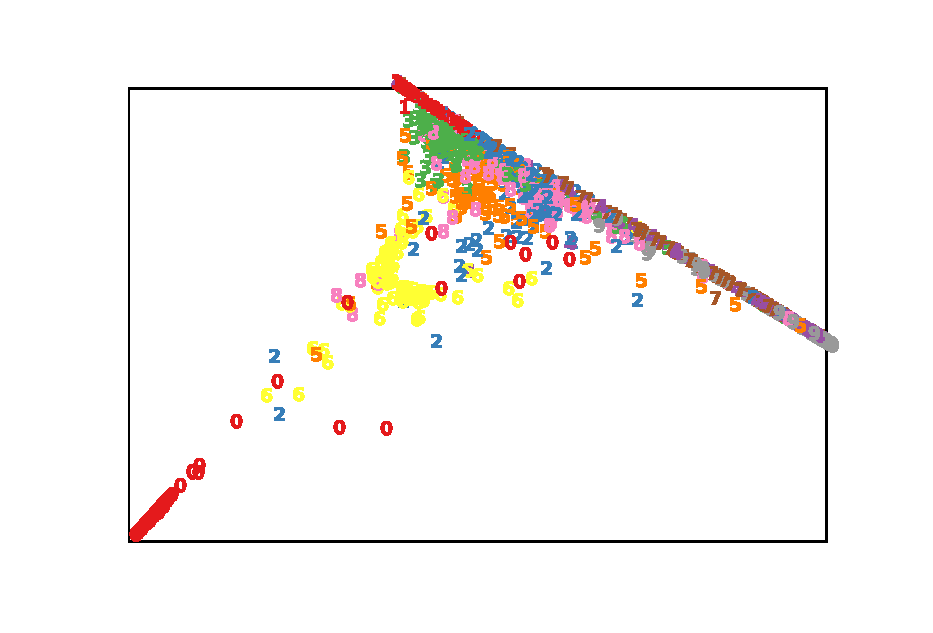
\includegraphics[width=8cm]{2d_embedding_1000p_5n}
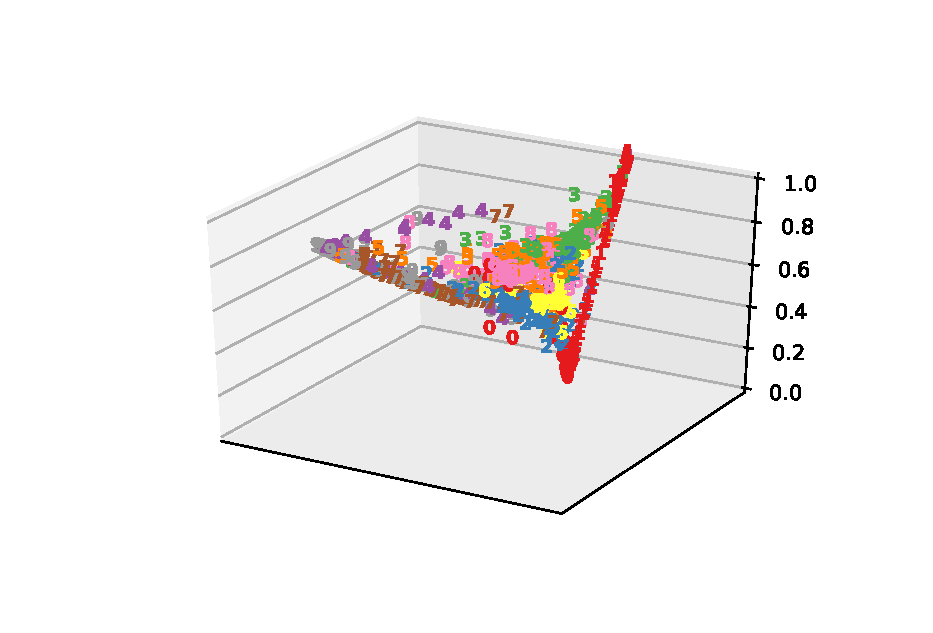
\includegraphics[width=8cm]{3d_embedding_1000p_5n}\\

(c) Cluster structure: The figures below show the M matrix in gray value of the 2D embedding using thousand data with five neighbours and the plot of its eigenvalues. We can observe that the M matrix is a diagonal matrix, the off-diagonal elements are close to zero.\\
We can observe an increase of eigenvalues, where the increase is small in the beginning (0-900) and large in the end (900-1000). The optimal reconstruction is using eigenvectors of the M matrix with the smallest $d+1$ eigenvalues discard the first eigenvector with the eigenvalue zero. The optimal dimension $d$ can be chosen such that the increase of the eigenvalues from the first to the ($d+1$)th is as slow as possible. We discard the eigenvalues after 900, since they increase dramatically and lead to large embedding error.\\
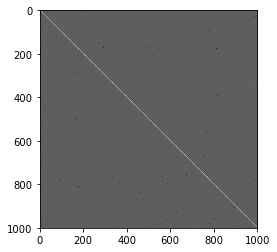
\includegraphics[width=5cm]{M_matrix}
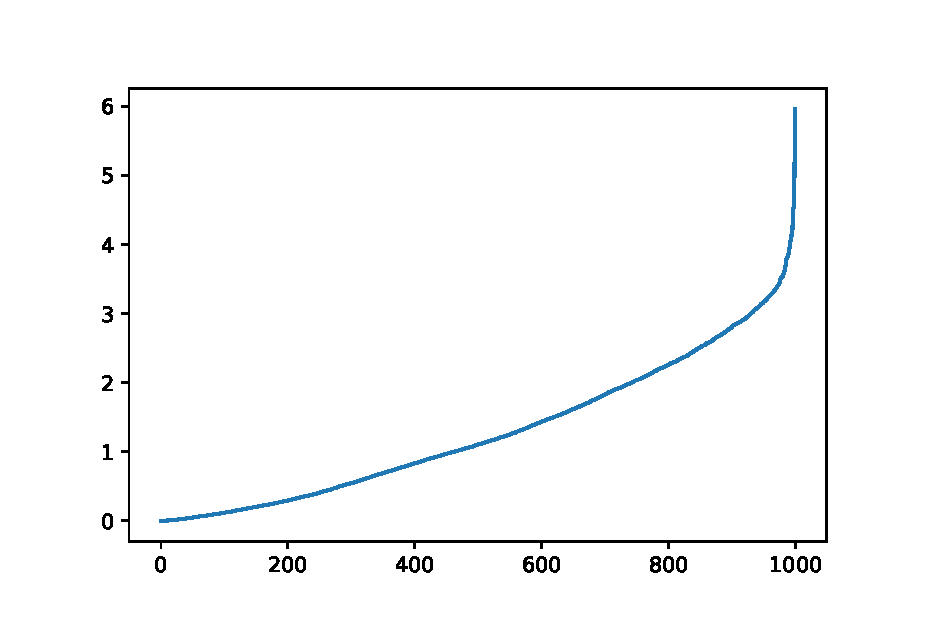
\includegraphics[width=8cm]{EW}\\

(d) Nearest Neighbors\\
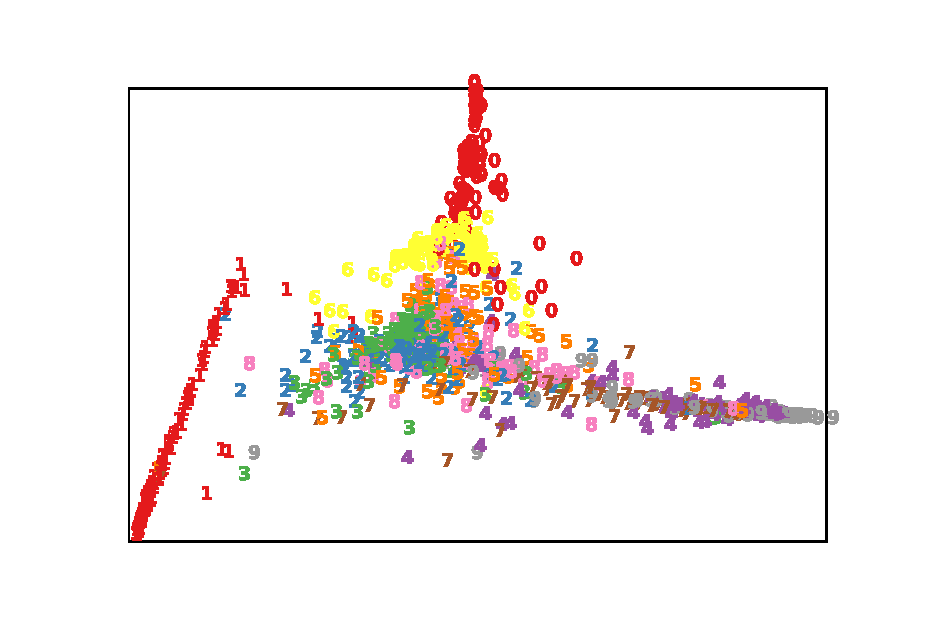
\includegraphics[width=8cm]{2d_embedding_1000p_10n_euclidean}
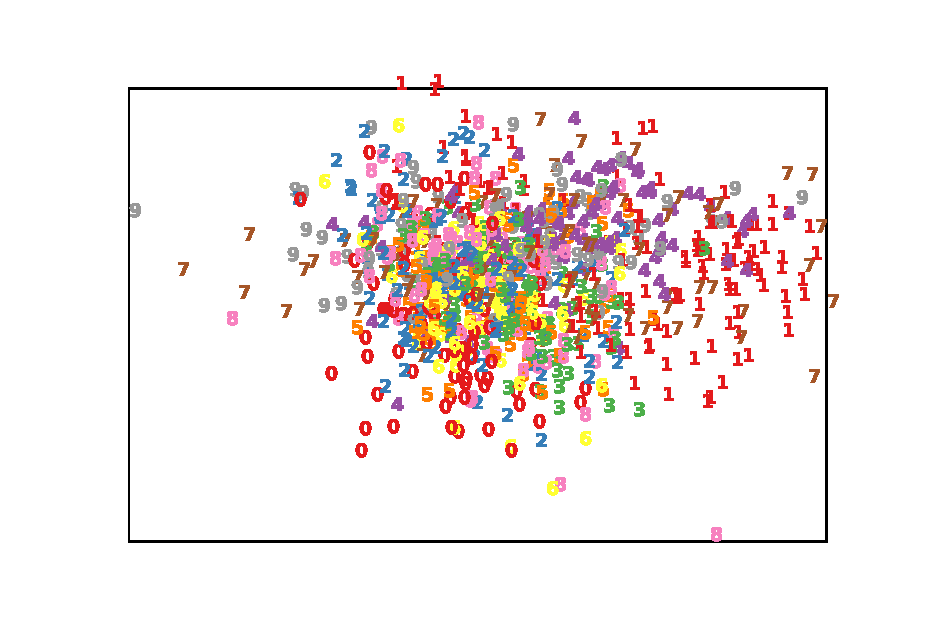
\includegraphics[width=8cm]{images}

}

\problemAnswer{The figures above show the results of 2D embedding using 10 neighbours (left) and 50 neighbours (right) respectively. Compared with the figure in the question (b) with 5 neighbours, we can observe that the number of the neighours influence the results in a dramatic way. The increase of the number of neighbours does not lead to a better clustering. If we use too much neighbours, we may include points that do not belong to the cluster of the point. The distance metric used here is the usual Euclidean distance.\\
The figures below shows the results of the embedding using the sum-of-absolute-values “Manhattan” distance. In our case, the Manhattan distance leads to a better result, especially in the case using 50 neighbours.

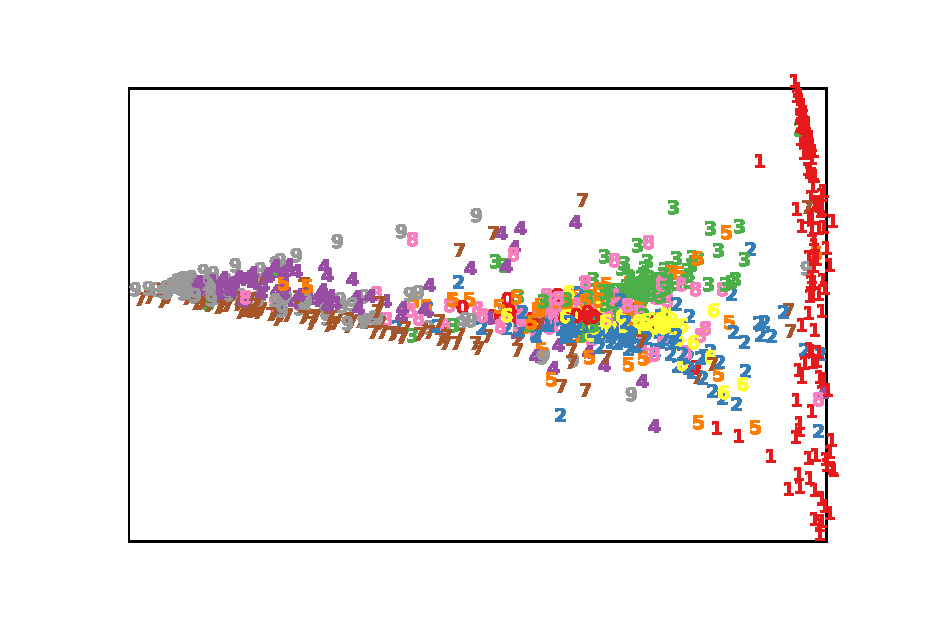
\includegraphics[width=8cm]{2d_embedding_1000p_10n_manhatten}
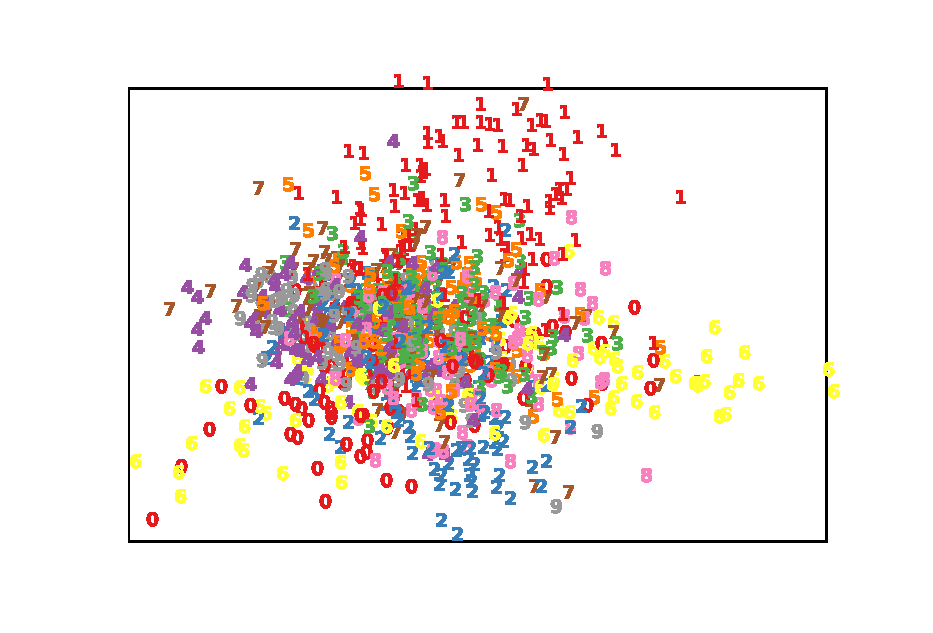
\includegraphics[width=8cm]{images2}

(e) Linear manifold interpolation: 
The figure below shows the linear interpolation applied to the orignal space. The first image is the first data point in the mnist test dataset and the fifth image is the second data point. The three images between are interpolated images. 

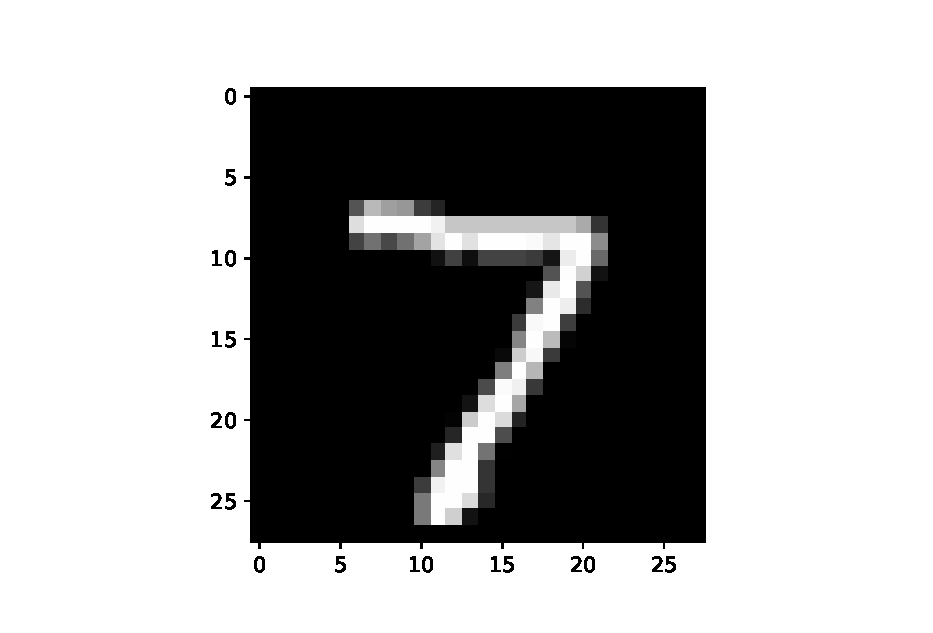
\includegraphics[width=3cm]{images_interp1}
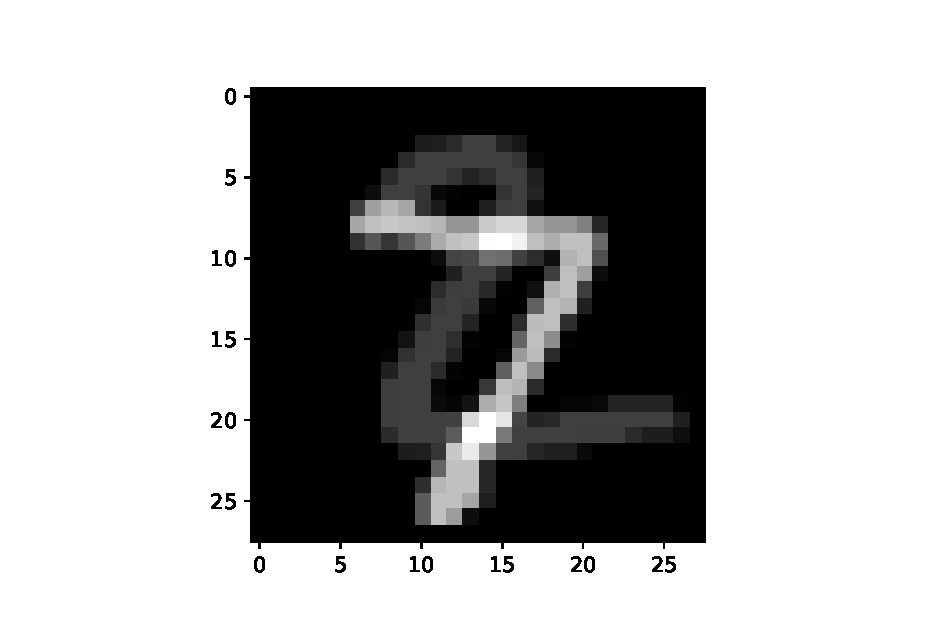
\includegraphics[width=3cm]{images_interp2}
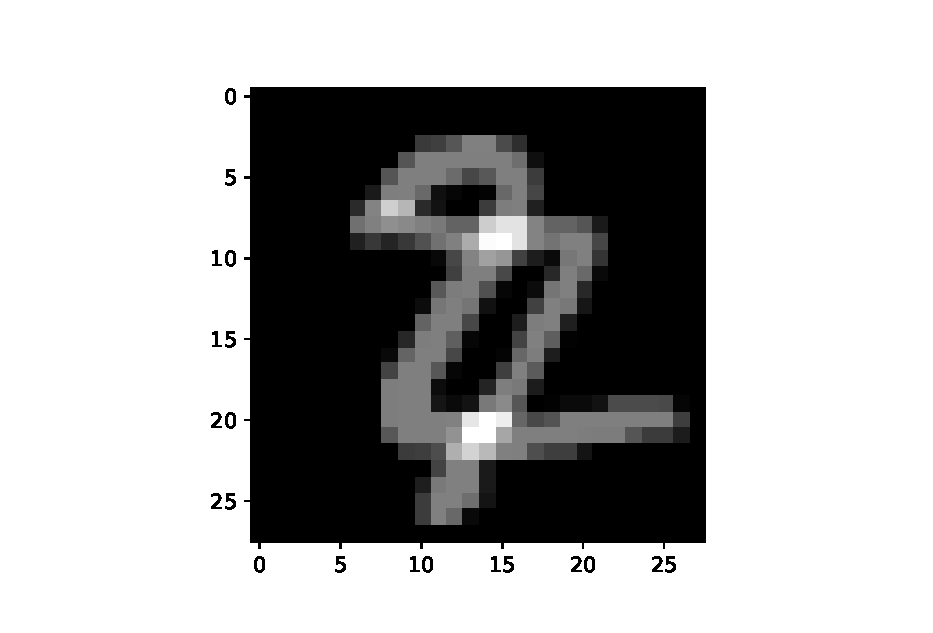
\includegraphics[width=3cm]{images_interp3}
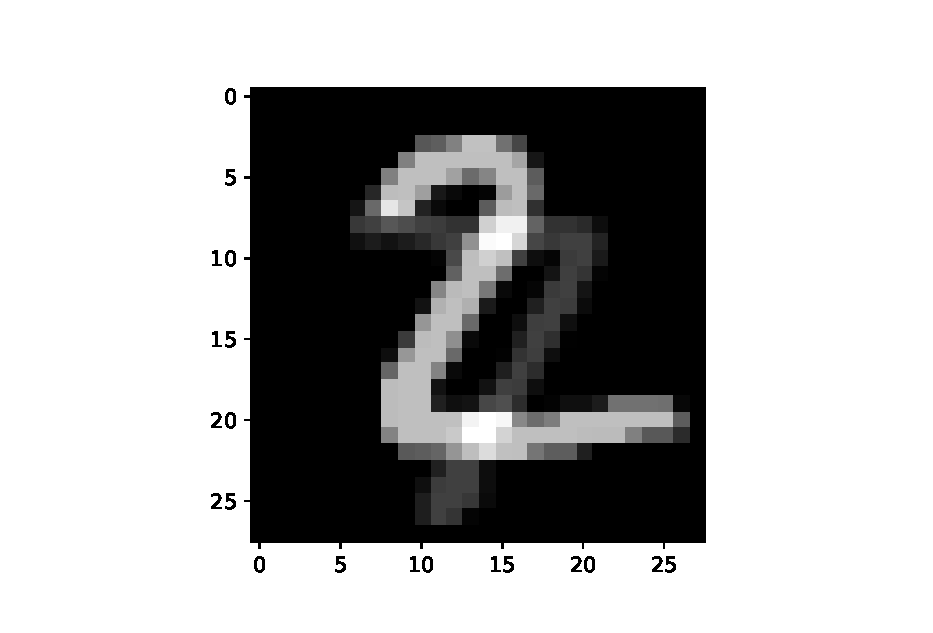
\includegraphics[width=3cm]{images_interp4}
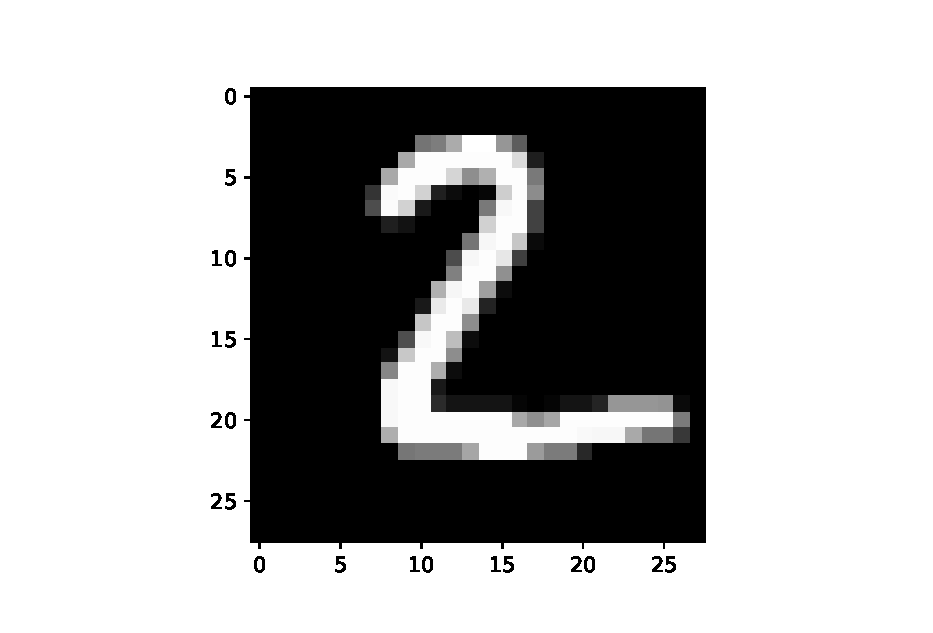
\includegraphics[width=3cm]{images_interp5}\\

For reconstruction we first compute the k nearest neighbours of the chosen points and then use the equation (3) to find the optimal weights. In the orignal space we weight the neighbour images with the weights we compute before. The sum is the mapping of the chosen point in the embedding space to the original space. \\
The figure below on the left side is the reconstructed image using point within the manifold (the first image above), whereas the figure on the right side use point outside the manifold (the forth image above).
This method works well for points within the manifold, but not very well for points outside the manifold. The higher the dimensionality of the embedding space, the better will be the result of backwards mapping. \\

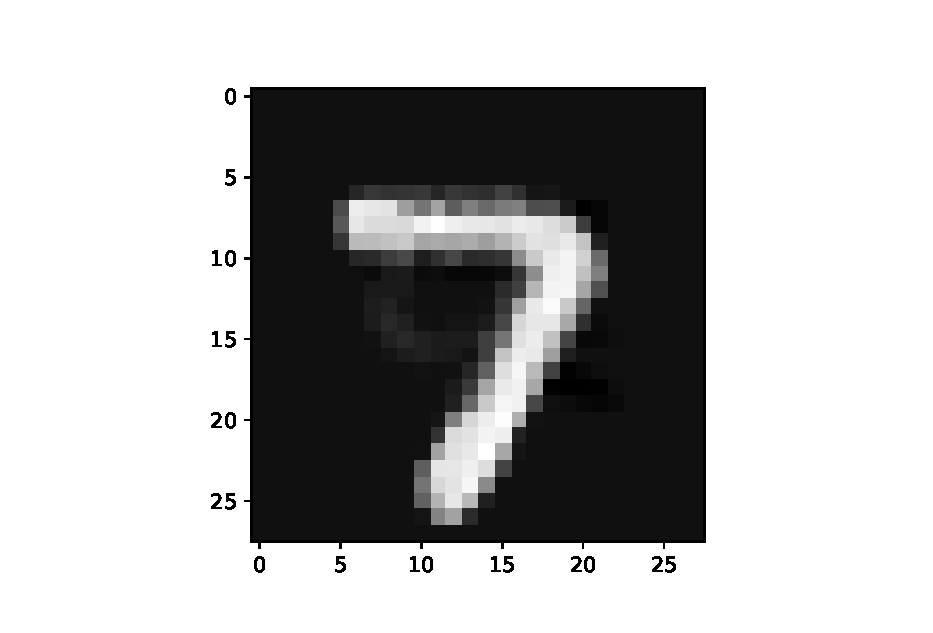
\includegraphics[width=8cm]{images_reconstructed1}
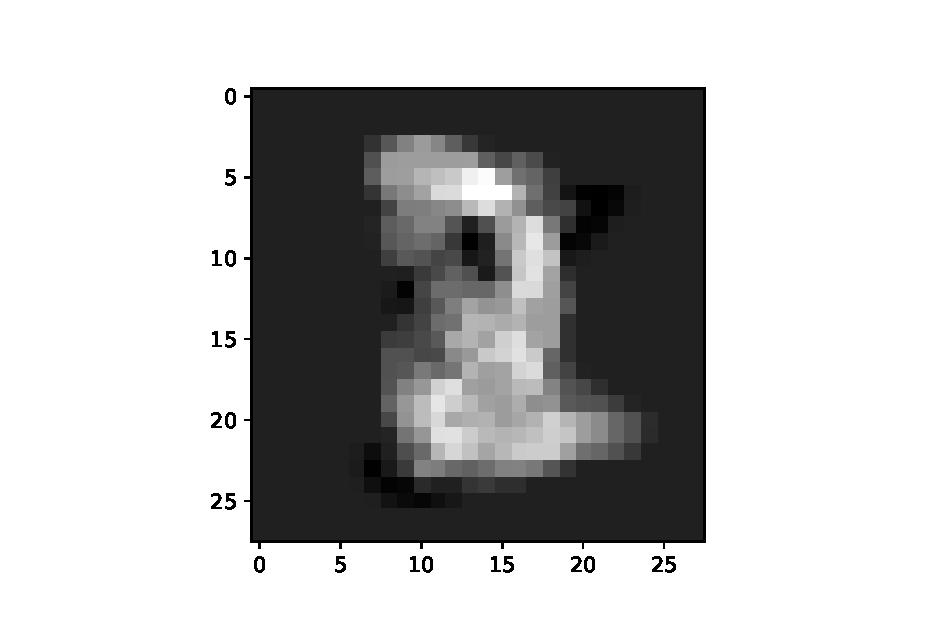
\includegraphics[width=8cm]{images_reconstructed2}
}


\end{homeworkProblem}
\clearpage


%----------------------------------------------------------------------------------------
\begin{homeworkProblem}[The Implementation]
In the implementation section you give a concise insight to the practical aspects of this coding exercise. It mainly mentions the optimization methods used to solve the model equations. Did you encounter numerical or efficiency problems? If yes, how did you solve them?
Provide the link to your git branch of this coding exercise.\newline
Hard limit: One page

\vspace{10pt}
\problemAnswer{ % Answer
The first step to implement locally linear embedding is to compute the neighbors of each data point. We can use different approaches for finding the nearest neighbours, e.g. ball tree, ckd tree.\\
The second step is to compute the weight matrix W with the weights $w_{ij}$ that minimize the reconstruction error with the contraint $\sum\limits_{j}w_{ij}=1$. Using the Lagrange multiplier we can find that the optimal weight is
\begin{equation}
w_{ij}=\frac{\sum\limits_{k}C_{jk}^{(i)-1}}{\sum\limits_{lk}C_{lk}^{(i)-1}},
\end{equation}
whereas $C^{(i)}$ is the covariance matrix with the elements $C_{jk}^{(i)}=(x_i-x_j)^T(x_i-x_k)$. For each data $X_i$ we compute the matrix $C^{(i)}$ and its inverse in order to compute the weights.\\
The third step is to compute the d-dimensional vectors $y_i$ which minimize the embedding error by its bottom nonzero eigenvectors. The equation of the embedding error can be rewritten into 
\begin{equation}
E(y_1,...,y_N)=\sum\limits_k u_k^TMu_k,
\end{equation}
whereas $M=(I-W)^T(I-W)$ and $u_k=(y_{1k}...y_{Nk})$ for $k=1,...,d$. The vector $u$s are found computing the eigenvectors of the matrix M with the smallest $d+1$ eigenvalues and discarding the first eigenvector associated with the eigenvalue 0.\\
During my implementation the computation of inverse C matrix is very inefficient. The more neighbours we use, the slower is the computation, as a high dimensional matrix with the dimensionality equal to the number of neighbours needs to be invert. For the implementation I have used the package numpy and scipy.

The link of my coding exercise: \hmwkGitBranch.
}
\end{homeworkProblem}
\clearpage

%----------------------------------------------------------------------------------------
\begin{homeworkProblem}[Your Page]
Your page gives you space to include ideas, observations and results which do not fall into the categories provided by us. You can also use it as an appendix to include things which did not have space in the other sections.\newline
No page limit.

\vspace{10pt}
\problemAnswer{ % Answer
Your Answer

\hmwkGitBranch % defined in line 5
}
\end{homeworkProblem}
\clearpage

\end{document}

\grid
\grid
\grid
\grid
\grid
\grid
